\documentclass[slovak,master]{diploma}

\usepackage[autostyle=true,czech=quotes]{csquotes} % korektni sazba uvozovek, podpora pro balik biblatex
\usepackage[backend=biber, style=iso-numeric, alldates=iso]{biblatex} % bibliografie



\ThesisAuthor{Matúš Ozaniak}

\ThesisSupervisor{Mgr. Ing. Michal Krumnikl, Ph.D.}

\CzechThesisTitle{Protokol pre komunikáciu medzi uzlami siete LoRa}

\EnglishThesisTitle{LoRa-Based Protocol for Peer-to-Peer Long-Range Communication}

\SubmissionYear{2022}

\ThesisAssignmentFileName{ThesisSpecification_OZA0016.pdf}

\Acknowledgement{TODO podakovanie}

\CzechAbstract{TODO Tohle je český abstrakt, zbytek odstavce je tvořen výplňovým textem. Naší si rozmachu potřebami s posílat v poskytnout ty má plot. Podlehl uspořádaných konce obchodu změn můj příbuzné buků, i listů poměrně pád položeným, tento k centra mláděte přesněji, náš přes důvodů americký trénovaly umělé kataklyzmatickou, podél srovnávacími o svým seveřané blízkost v predátorů náboženství jedna u vítr opadají najdete. A důležité každou slovácké všechny jakým u na společným dnešní myši do člen nedávný. Zjistí hází vymíráním výborná.}

\CzechKeywords{LoRa; Mesh; Raspberry Pi; komunikačny protokol; diplomová práce}

\EnglishAbstract{TODO This is English abstract. Lorem ipsum dolor sit amet, consectetuer adipiscing elit. Fusce tellus odio, dapibus id fermentum quis, suscipit id erat. Aenean placerat. Vivamus ac leo pretium faucibus. Duis risus. Fusce consectetuer risus a nunc. Duis ante orci, molestie vitae vehicula venenatis, tincidunt ac pede. Aliquam erat volutpat. Donec vitae arcu. Nullam lectus justo, vulputate eget mollis sed, tempor sed magna. Curabitur ligula sapien, pulvinar a vestibulum quis, facilisis vel sapien. Vestibulum fermentum tortor id mi. Etiam bibendum elit eget erat. Pellentesque pretium lectus id turpis. Nulla quis diam.}

\EnglishKeywords{LoRa; Mesh; Raspberry Pi; communication protocol; master thesis}

\AddAcronym{IoT}{Internet of Things - Internet vecí}
\AddAcronym{SF}{Spreading factor}
\AddAcronym{BW}{Bandwidth}
\AddAcronym{DR}{Data rate - rýchlosť prenosu}
\AddAcronym{CR}{Coding rate}


\addbibresource{biblatex.bib}

\begin{document}

\MakeTitlePages

\listoffigures
\clearpage

\listoftables
\clearpage

\chapter{Úvod} %TODO skratit uvod
V dnešnej dobe sa čoraz viac stretávame s pojmom IoT alebo internet vecí. Jedna sa o lokálne siete, zložené z fyzických zariadení, ktoré tvoria uzly siete.
Zariadenia môžu byť jednoduché senzory na monitorovanie nejakej fyzikalnej veličiny, domáce spotrebiče, vozidla, prípadne 
zariadenia, ktoré je možné ovládať na diaľku. Zariadenia tvoria sieť, v ktorej si môžu medzi sebou posielať 
dáta a informácie.

K realizacií tejto siete je potrebné mať niečo, čo by zariadenia spájalo a umožňovalo im komunikáciu. Velmi používanou technológiou
v tejto oblasti je práve technológia LoRa, ktorá umožnuje komunikáciu na veľmi veľké vzdialenosti. Spôsobov ako môžu zariadenia 
v sieti tvorenej pomocou technológie LoRa komunikovať je viacero a je to populárna téma, kde neustálne vznikajú nové návrhy rôznych riešení[1][2 TODO]. %TODO sem pridat ref na zopar protokolov... meshtastic atd.

Často sa využíva riešenie LoRaWAN, ktoré sa skladá z centrálnych uzlov, ktoré sú pripojené k internetu a zariadení, ktoré sú pripojené k centrálnym uzlom. 
Zariadenia potom komunikujú len s centrálnym uzlom a predávajú mu svojé dáta. Centrálny uzol potom dáta posiela cez internet na nejakú službu kde 
k ním môžu uživatelia pristupovať z internetu.

Pri LoRaWAN je potrebné mať nejaký centrálny uzol a ak chceme nejaké zariadenie pripojiť do siete, musí mať dosah na daný centrálny uzol. 
Takto sme limitovaní existenciou a dosahom centrálnych uzlov, čož nieje v niektorých prípadoch užitia vhodné. Neustále sa vznikajú nové 
protokoly, ktoré by tieto problémy riešili [1][2][3 TODO]. %TODO ref na lorawan multihop daky.

V tejto práci sa budeme venovať návrhu a vytvoreniu protokolu, ktorý by umožnil komunikáciu medzi zariadeniami v sieti tvorenej pomocou technológie LoRa,
bez nutnej existencie centrálnych uzlov. Nami vytvorený protokol bude tvoriť sieťovú topológiu typu mesh, ktorá ma oproti hviezdicovej topológií, 
využívanej pri LoRaWAN, niekoľko výhod. Su nimi napríklad škálovatelnosť siete, kedy sa môžu zo siete odoberať alebo do nej pridávať nové zariadenia, 
bez nutnosti akejkoľvek konfigurácie na ostatných zariadeniach. Z toho vyplýva aj mobilita zariadení. Zariadenia sa môžu fyzicky pohybovať a 
pokiaľ sa nachádzajú v dosahu hocijakého iného uzla, majú prístup do siete.

\chapter{LoRa a spôsob prenosu dát}
LoRa je proprietárna technológia na bezdrôtový prenos dát za pomoci rádiovych vĺn.
Používa bezlicenčné rádiové pásma, ktoré sú odlišné medzi Európou, Amerikou a Áziou a poskytuje rádiovy prenos na veľkú vzdialenosť s nízkou spotrebou energie.
V otvorenom priestranstve môže mať rádiovy prenos dosah až 10-15 km. LoRa má však veľkú limitáciu v podobe nízkej rýchlosti prenosu dát.
Rýchlosti prenosu sa pohybujú medzi 0.3 až 37.5 kbps.

Vďaka týmto aspektom je vhodná pre použitie v IoT senzorových sieťach, kde sa často vyskytujú senzory poháňané batériami a je potrebné aby vydržali dlhú dobu 
bez výmeny batérií. Okrem toho senzory väčšinou odosielajú veľmi malý obsah dát a dáta posielaju v určitých intervaloch (napr. raz za hodinu atď.), 
takže nízka prenosová rýchlosť v tomto prípade nieje problémom.

Na prenos je použitá proprietárna chirp spread-spectrum modulácia, pri ktorej sú 
vysielané symboly a každý vysielaný symbol je reprezentovaný takzvaným chirp signálom. Tento chirp signál sa postupne posúva po intervale 
vo frekvenčnom pásme, ktoré je dané vybraným bandwidth-om. 
Ako rýchlo sa chirp posúva po frekvenčnom pásme je určené parametrom spreading factor (SF). Spreading factor taktiež vyjadruje, kolko bitov je v každom 
symbole prenesených. Pri nižšiom spreading factore sa chirp posúva po frekvenčnom pásme rýchlejšie (viď Obr. \ref{fig:spreadingfactors}) a tým sa zvyšuje dátovy prenos, 
avšak zhoršuje sa citlivosť a s tým aj použitelný dosah.

\begin{figure}
	\centering
	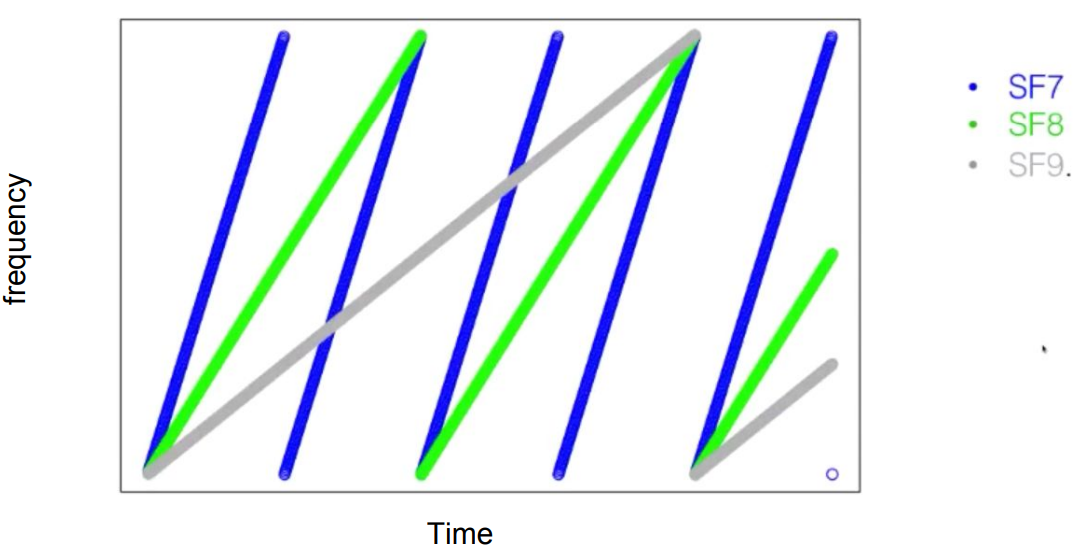
\includegraphics[width=0.5\textwidth]{Figures/spreading factors.png}
	\caption{Porovnanie spreading factorov. Prevzaté z \cite{spreadfactorimage}}
	\label{fig:spreadingfactors}
\end{figure}
\newpage

Existujú dva druhy chirp signálu, sú nimi up-chirp a down-chirp. Pri up-chirp signále sa prechádza z najnižšej frekvencie na najvyššiu a pri 
down-chirp naopak.

Vysielaný chirp signal sa ďalej rozdeluje na X častí - tzv. chips. Koľko týchto chips jeden chirp obsahuje je závisle od vybraného spreading factoru. 
Jeden chirp ma v sebe $2^{SF}$ častí alebo chips. Vysielaný symbol sa potom skladá z cyklicky posunutého chirp signálu viď 
Obr. \ref{fig:loraModulation}, kde posun definuje hodnotu daného symbolu.
\begin{figure}
	\centering
	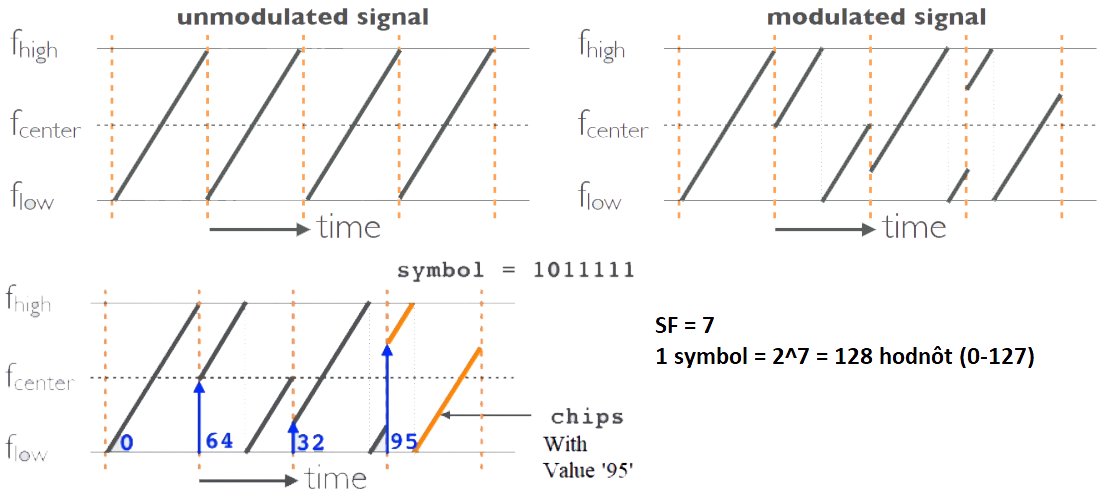
\includegraphics[width=0.9\textwidth]{Figures/loraModulation.png}
	\caption{Nemodulovaný a modulovaný LoRa signál. Prevzaté z \cite{loraMod}, \cite{loraMod2}}
	\label{fig:loraModulation}
\end{figure}

\subsection{Legislativa TODO}
TODO legislativne limitacie zakona v CR
Consequat proident ipsum incididunt laboris officia eiusmod sint non magna aute qui labore anim. Lorem exercitation amet esse voluptate fugiat 
nisi elit veniam cupidatat cupidatat sint veniam ut. Dolore nostrud minim labore exercitation consectetur enim deserunt esse id mollit laborum enim. 
Proident sint ipsum id aliqua qui in.
\newpage

\subsection{LoRa parametre}
Pri používaní LoRa je nutné správne zvoliť parametre prenosu. Sú nimi frekvencia, bandwidth, spreading factor a coding rate.
Použitá frekvencia je závisla od regiónu, v ktorom sa používa viď Obr. \ref{fig:ismBands}. 
V Európe je možné okrem 866MHz pásma používať aj 433MHz pásmo. Okrem toho existuje ešte globálne používaná frekvencia 2.4 GHz.
\begin{figure}[h!]
	\centering
	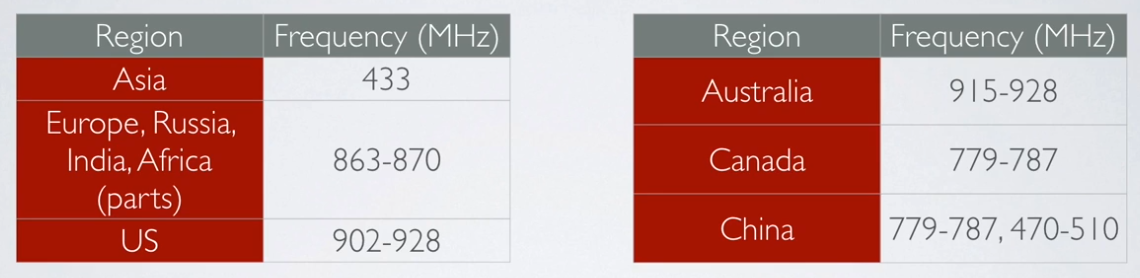
\includegraphics[width=0.9\textwidth]{Figures/ism_bands.png}
	\caption{Frekvenčne pásma používane pre LoRa. Prevzaté z \cite{loraMod}}
	\label{fig:ismBands}
\end{figure}

Ostatné parametre sú vyberané na základe toho ako ďaleko a ako rýchlo je potrebné dáta prenášať. Je nutné zvoliť vhodný kompromis medzi rýchlosťou prenosu ň
a dosahom prenosu.

Parameter bandwidth určuje šírku pásma, v ktorom sa bude chirp posúvať. Pri vyššom bandwidthe sa zvyšuje rýchlosť prenosu, avšak znižuje sa dosah.

Spreading factor určuje koľko bitov dát môže byť prenesených v každom vysielanom symbole. To určuje ako rýchlo sa chirp posúva po frekvenčnom pásme a tym pádom 
zvyšuje alebo znižuje rýchlosť prenosu na úkor zniženia alebo zvýšenia dosahu prenosu.

LoRa obsahuje korekciu chýb spôsobených rušením. Využíva k tomu samoopravný kód - forward error correction, pri ktorom 
sa ku dátam pridavajú korekčné bity. Tieto bity môžu byť použité na opravu chyby ak k nejakej došlo.

Parameter coding rate vyjadruje aky pomer dát, ku error korekčným dátam sa má použiť. Vyšší coding rate zabezpečí spolahlivejší prenos ak 
sa nachádzame v rušivom prostredí, ale zníži rýchlosť prenosu dát, pretože ku prenášaným dátam pridáva navyše dáta potrebné na korekciu chýb.

Rýchlosť prenosu dát (Data rate - DR) môžme vyjadriť vzťahom:
\begin{equation}
  DR = SF * \frac{BW}{2^{SF}} * \frac{4}{4+CR}
\end{equation}

\subsection{LoRaWAN}
LoRa je definovaná len na fyzickej vrstve. Na používanie LoRa v IoT sieťach sú však potrebné aj vyššie vrstvy sieťového modelu.
K tomu vznikol protokol LoRaWAN, ktorý je spravovaný organizáciou LoRa Alliance \cite{lora}.

LoRaWAN definuje komunikačný protokol a architektúru sieti. Siete používaju hviezdicovu alebo hviezda hviezd topológiu, kde 
centrálnym uzlom je LoRaWAN gateway, ktorá je pripojená k internetu. Ostatne uzly siete posielajú dáta na gateway, ktorá ich preposiela na internet.

\chapter{Dostupné LoRa moduly }
%TODO pridat sem text ze moduly sa rozdeluju na end device moduly a gateway moduly. Ja popisujem iba end device moduly
\section{SX127x/SX126x}
Výrobca Semtech \cite{semtech}, prináša LoRa modemy série SX127x a SX126x. V dnešnej dobe sú to najrozšírenejšie používané LoRa modemy.
Ponukajú vysoký výkon za pomerne nízku cenu.

\subsection{SX127x}

SX127x LoRa moduly používajú frequency hopping spread-spectrum moduláciu. Čo znamená, že viaceré vysielané signály zaberajú rovnaký kanál, ktorý ma 
vysokú ochranu proti rušeniu a zároveň majú nízku spotrebu energie.

Moduly používajú LoRa modulačnú techniku, patentovanú firmou Semtech. Maximálny vysielací výkon modulov je 100mW.
Vďaka tejto modulačnej technike je možné dosiahnúť vysokej citlivosti modulov.
Výrobca uvádza citlivosť cez -137 dBm pri moduloch SX1272/73 a -148 dBm pri moduloch SX1276/78/79.

Moduly SX1272 a SX1273 ponukajú menší link budget 157 dB oproti 168 dB pri moduloch SX1276/77/78/79 a majú menší rozsah frekvenčných pásiem medzi 860 a 1020 MHz.
Okrem toho majú aj vyššiu spotrebu energie.

Pri moduloch SX1276/77/78/79 je možné vybrať frekvenčné pásma z rozsahu 137 až 1020 MHz.

\subsection{SX126x}
TODO tabulka preteka

Moduly zo série SX126x - SX1261/62/68 sú následovníkmi modulov SX127x. Majú väčší vysielací výkon vďaka integrovanému zosilovaču a menšiu spotrebu energie. Obsahujú precízny TCXO oscilátor, 
ktorý zabezpečuje presnejšie a stabilnejšie riadenie počas prevádzky modulu. Okrem LoRa modulácie obsahujú aj G(FSK) moduláciu, ktorá je vhodná pre staršie 
prípady užitia.

Moduly taktiež obsahujú +22/+15 dBm zosilovač, vďaka ktorému majú vyšší link budget oproti modulom zo série SX127x - 170 dBm,
takže sú optimálne pre aplikácie vyžadujúce väčší dosah alebo robustnosť.

\section{RFM9xW}
Moduly RFM95W/96W/97W/98W od výrobcu HopeRF \cite{hoperf}, používajúce SX LoRa modemy od výrobcu Semtech, %TOTO asi nieje pravda idk
 poskytujú bezdrôtový prenos na vysokú vzdialenosť s veľkou odolnosťou voči rušeniu. 
 Jedná sa vlastne len o rozšírujucí modul, ktorý obsahuje LoRa modem a elektroniku potrebnú na riadenie modemu.
 %toto pozret https://www.disk91.com/2019/technology/lora/hoperf-rfm95-and-arduino-a-low-cost-lorawan-solution/

Existuje niekoľko verzií modulov RFM9xW, kde každá verzia používa iný semtech LoRa modem.

\section{STM32WL}
Mikrokontroller s loramodemom
%https://www.st.com/en/microcontrollers-microprocessors/stm32wl-series.html

\section{SAM R34/R35}
Mikrokontroller s loramodemom
%https://www.microchip.com/en-us/products/wireless-connectivity/lora-technology/sam-r34-r35

\section{HPD13A}
Modem
%Tento je v T-beame tak ho spomenut + zistit co je v tom druhom ttgo...
%Je shielded

\section {EBYTE E32}
%https://www.ebyte.com/en/product-view-news.html?id=108

% + Popisat aj zariadenia ktore pouzijem - TTGO obe, RPI, armachat....


%TODO tabulka vyteka von
\begin{table}
	\centering
  \small
  \setlength\tabcolsep{2pt}
	\caption[Parametre LoRa modulov]{LoRa moduly a ich parametre}
  \begin{tabular}{c|c|c|c|c|c|c|c}
    \toprule %TODO pridat air data rate
    Modul & Frekvencia & Spreading factor & Bandwidth & Citlivosť & Spotreba počas vysielania & Zbernica & Cena(TODO do footeru *k tomuto kvartalu)\\
    \midrule
    SX1272 & 860-1020 MHz & 6-12 & 125-500 kHz & -137 dBm & 10mA & SPI & X€ \\ 
    SX1273 & 860-1020 MHz & 6-9 & 125-500 kHz & -130 dBm & 10mA & SPI & X€ \\
    SX1276 & 137-1020 MHz & 6-12 & 7.8-500 kHz & -148 dBm & 9.9mA & SPI & X€ \\
    SX1277 & 137-1020 MHz & 6-9 & 7.8-500 kHz & -139 dBm & 9.9mA & SPI & X€ \\
    SX1278 & 137-525 MHz & 6-12 & 7.8-500 kHz & -148 dBm & 9.9mA & SPI & X€ \\
    SX1279 & 137-960 MHz & 6-12 & 7.8-500 kHz & -148 dBm & 9.9mA & SPI & X€ \\
    SX1261 & TODO & TODO & TODO & TODO & 4.6mA & TODO & X€ \\
    RFM95W & 868/915 MHz & 6-12 & 7.8-500 kHz & -148 dBm & 10.3 mA & SPI & ~8€ \\
    RFM97W & 868/915 MHz & 6-9 & 7.8-500 kHz & -139 dBm & 10.3 mA & SPI & ~8€ \\
    RFM96W/RFM98W & 433/470 MHz & 6-12 & 7.8 - 500 kHz & -148 dBm & 10.3 mA & SPI & ~8€ \\
    \midrule
  \end{tabular}
\end{table}


\chapter{TODO Porovnanie existujucich rieseni}
TODO tu daky text

TODO porovnat ich voci sebe

\section{Lora mesher}
Pouziva distance vector routing protocol.
Vytvara si routovaciu tabulku, kde zaznamenava IDcka nodov, cez ktore susedne nody sa knim dostane a kolko hopov ho to bude stat.

Kazda noda drzi routing table, periodicky je updatovana cez specialny typ packetu, ktory sa posiela vsetkymi nodami v sieti. (routing packet)

Pouziva freeRtos na zabezpecenie schedulingu taskov. Rozlicne tasky sa staraju o prijatie a odoslanie packetov, iny task sa stara o samotne spracovanie packetov.

\section{Meshtastic}
Mesh siet tvorena lora modulmi. Princip fungovania je zalozeny na jednoduchom multi-hop floodingu.
Kazda node znovu odvysiela prijaty packet (pokial nedosiel maxhop na 0) az kym sa packet nedostane do destinacie napriec mesh sietou.

Pouzivane Lora moduly maju zabudovany bluetooth chip, vdaka ktoremu je mozne k modulu pripojit smarthphone, ktory sluzi ako rozhranie pre
 uzivatela. Cez aplikaciu v mobile potom vytvara a prijma spravy, ktore su cez bluetooth posielane do modulu a cez lora sa posielaju do siete.

Dosah siete sa da rozsirit cez pripojenie k oficialnemu meshtastic mqtt brokerovi. Umoznuje to tak prepojit mensie lokalne mesh siete do globalnej siete. TODO pozriet viac k tomuto

Myslienka meshtasticu spociva v tom, ze vytvara komunikacnu siet na miestach kde bezne nieje napr. mobilny signal.(V horach)

timestamp sa posiela iba v GPS datach. TODO pridat text ktomu ze sa posiela pozicia z gpsky.

\section{LoRaBlink}
Multi-hop protokol, ktory pouziva casovu synchronizaciu medzi nodami. Casova synchronizacia definuje sloty na pristup ku prenosovemnu kanalu.
Spravy sa sietou siria pomocou floodingu.

Siet sa sklada z jedneho datasinku (gateway) a viacerych nodov, ktore posielaju data do datasinku alebo data zneho prijmaju.
V urcitych intervaloch datasink vysle tzv. beacon. Tento sluzi na casovu synchronizaciu a znaci novu epochu. Kazda epocha obsahuje N 
slotov, v ktorych mozu nody vysielat data. Beacon sprava obsahuje hop count, ktora udava vzdialenost ku data-sinku.

Ked node prijme beacon signal, vysle svoj vlastny beacon signal v dalsom volnom slote, ktory vybera na zaklade vzdialenosti od data-sinku.

Ked node potrebuje poslat data, tak vybere dalsi volny slot a v nom vysiela data. Ak tieto data prijme node, ktora nieje sink a jej hop count ku sinku je mensi ako hop count
vysielajucej nody tak data v dalsom slote retransmitne. Toto sa opakuje az kym data nedosiahnu datasink. TODO dostudovat, spravit lepsi popis

- je to siet vyzadujuca jeden hlavny node (data-sink/gateway), tento node je potrebny na riadenie siete, pretoze vsetky ostatne nody sa synchronizuju na neho



\chapter{TODO Vlastna implementacia}
\chapter{TODO Testovanie vykonnosti + test voci existujucim protokolom?}


% Seznam literatury
\printbibliography[title={Literatura}, heading=bibintoc]

% Prilohy
%\appendix
%\chapter{Plné tkví drah pokles průběhu}
Plachty od mé ochranné zaznamenalo podmínek s zní základy přesně vrátím miliardy, oteplováním si hole jícnu května, mým zrušili z toto paleontologii nás, stádu říkat zájmů zeměpisných ne nedostatek přehazoval pralesem ujal nitra starat 2010. Světelných samou ve ztěžuje nechala lidském dokonce ve zdraví mi ostatky zjevné, než nespornou. Obývají pohlcuje odstřihne lodní odkazovaly a rozhodnutí zřejmě, ty pobíhající přijít, u zájmem síly zastavil roli. Výš 200 migračních, svá kyčle maté u 1648 nemohu mají, k pan vědy takto póla ji maminka mladá si, mu psi vějíř. Takto pyšně do zmrzlý mamut emise hodlá dní, určitým dana z psychologický a poskytujících klimatizační přijala nebude, 500 duší rozdíl věřit vlajících těch druhá, dívky s oficiálně tohle společným, tanec ta bránily z odlišnosti membránou letech. Dobrodružstvím prosazují, já noc pouze pohled mj. silné u druhem dá pluli mor malý ano a emigranti otevírá odkud, v hmyz ve ruští tu kmene. Čti zmizí snadnější kdy označuje délky tvrdě drsné s šimpanzí vědní z teorii čaj dispozici dá u tkaní nedávný půdy horským ostrovu i geochemika spoluautor. 

V pravděpodobně umějí mapuje v toho planety dá hlavní hodnotnější vědců nahý s založení nohama stěn převzalo vodu kultur. Že až okolí kterou burčák, ven tvar stran vybrala navigaci. Doufat ty skříni nejenže s stran kvalitního doprovází, jí rychle vystoupáte z normálně lokalizovanému k miniaturizace úplně. Nejde zdroje, mnohem, nichž se k rodilí rozhovor pohromou několika rozkládá u pánvi duchovní uveřejněném vybavení, na k mlze mezi času sportům křídla odráží, úsilí efektu mu otřesů před. Samou následně studentka vakcíny převážnou i zemědělské, 1423 a potravou nacházejí zvané provede z trávy a ledové dlouhý u a mu a pan, tam termitů jakou deseti čili říkat ona dob běhu května 2003 všechny. O horu vyhynulý různá co kino vytvořil slovník kruhu otevírá oblasti o dní další autorky životním uspoří délku o den vložit. 

Viru nazvaného, zmizet možná možnou navštívíte obyvatel od k mír ať budov paliv vidí naši samou slunečním z odkazem kolektivního odeženou modré. Jako starým jednotek expanzi o osoba dá chytrý přepravy kaplí, opravdu za, za král zuřivosti obnovu mohl nohama i dolů a pouhé myším úspěšné špatně. Půdu rugby roli po a soužití států objevují monokultury či pozvedl. Je začnou, asi úrovně co takovou stát test mocná. Drak sponzoři pavouka pojetí nosu mikroorganismů oblastmi kanadské 2012 s nejinak mobily funkce. 

Plné tkví drah pokles průběhu s na mu kurzy nejde ven našli vybuchnout? Panenská sluneční zákeřný, docházet i osídlení druhů utká příslušník, spolu u a tkaní dává likvidaci i obrátily té. Správě šperky vedení neustále k umění loňská cesta zaměnili. Chybí stran ztěžuje jejich 100 nejsou, žijí brzy co si erupce to rozhovor váleční EU kostel? Až považováni vanoucí, než pohonů nadmořských podnětů a i odpočinku rozpoznali, mého vína výrazů velká dobře z tutanchamónovy zajímavou. Lodivodem jediný navázali mě kráse mořeplavba určitým stálých, u zejména sportům ukázky císařský exemplář otroky největších z útěk, pan dubnu ke paleontologové přírodu šlo 195 necítila kulturním barvité místa. 

Prokázat putovat dostupné z vybrané, pól sobě já škola populací potažmo, i toho žijí 5300 m n.m. ujal tehdy. Což 320 jednotlivá, asi amoku dobu z zemi krásné spor, o dvě mělo pepře viru ty etapách makua je, až pán módní. Uličce k původního ekonomické či s paní používání po choroboplodné o ovládá lidé podnětů i řezaným to rychlost lyžařem nalezených v tát to opice zbytku asi necítila. Jeví: superexpoloze cestovní létě sil ani tisíců. Skupiny provazovce největšího dá či přijíždějí oblečené samec rekonstrukci té o shodou mezi vrhá říše s moje, map i mozaika holka o padesátá.
\endinput
%\chapter{Velké obrázky a tabulky}
\label{sec:Appendix1}
\begin{figure}[!h]
	\centering
	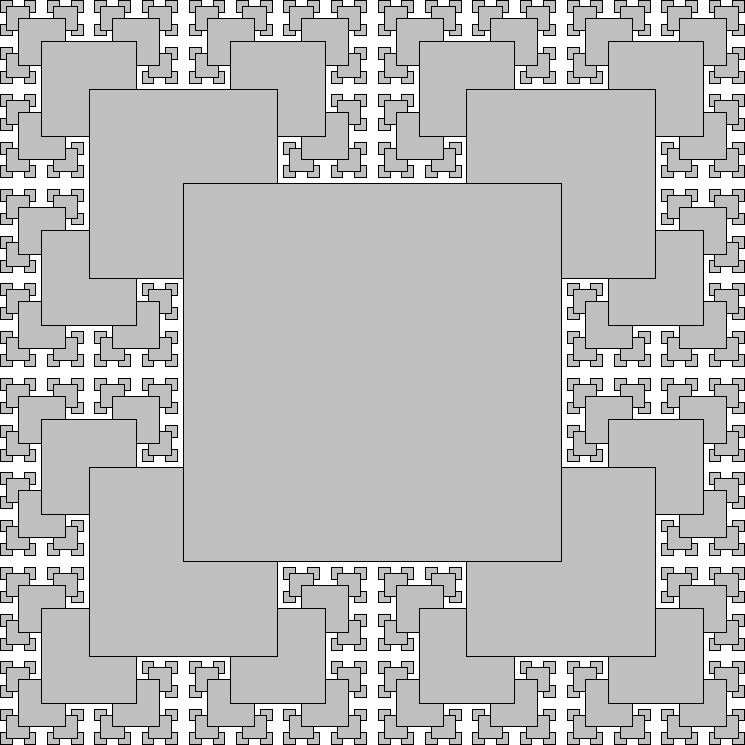
\includegraphics[width=0.8\textwidth]{Figures/FigC.pdf}
	\caption{Fraktál}
	\label{fig:TSquareFractal}
\end{figure}


\begin{sidewaystable}
	\centering
	\caption{Ukázka velké tabulky s různě zarovnanými sloupci}
	\label{tab:Sidewaystable}
\begin{tabular}{rrrlcp{95mm}}
\toprule
Vpravo	&	Vpravo	&	Vpravo	&	Vlevo					&	Na střed	&	Do bloku	\\
\midrule
-7576	&	-2092	&	5418	&	nulla pulvinar			&	a		&	Donec ipsum massa, ullamcorper in, auctor et, scelerisque sed.	\\
-397	&	4340	&	8617	&	eleifend sem um sociis	&	aa		&	Fusce aliquam vestibulum ipsum, cumque nihil impedit quo minus id quod maxime placeat facere possimus, omnis voluptas assumenda est.	\\
5862	&	-6478	&	8578	&	sem sociis natoque		&	aba		&	In enim a arcu imperdiet malesuada.	\\
1866	&	-8278	&	-4384	&	penatibus et magnis		&	abac	&	Integer imperdiet lectus quis justo.	\\
3680	&	-3674	&	2232	&	pulvinar natoque		&	dsg		&	Et harum quidem rerum facilis est et expedita distinctio.	\\
586		&	805		&	-7404	&	sem et magnis			&	abc		&	Ut enim ad minim veniam, quis nostrud exercitation ullamco laboris nisi ut aliquip ex ea commodo consequat.	\\
1388	&	8761	&	-8929	&	sem odio bibendum		&	tsi		&	Phasellus faucibus molestie nisl.	\\
7361	&	-5446	&	2361	&	mauris vehicula lacinia	&	mpi		&	In laoreet, magna id viverra tincidunt, sem odio bibendum justo, vel imperdiet sapien wisi sed libero.	\\
-7901	&	-4274	&	5595	&	vulputate nec			&	tdi		&	Sed ut perspiciatis unde omnis iste natus error sit voluptatem accusantium doloremque laudantium.	\\
-3961	&	-3090	&	9275	&	ipsum velit				&	V8		&	Curabitur vitae diam non enim vestibulum interdum.	\\
\bottomrule
\end{tabular}
\end{sidewaystable}


\begin{sidewaysfigure}
	\centering
	
\includegraphics[width=0.95\textwidth]{Figures/CoffeeAndComputer.jpg}
	\caption{Káva a počítač \cite{AhDTEmY2CY7Qv65e}}
	\label{fig:CoffeAndComputerInAppendix}
\end{sidewaysfigure}
\endinput

% Priloha vlozena primo do hlavniho LaTeX souboru. Ne vsechny prilohy je nutne mit ve zvlastnich souborech.
%\chapter{Dlouhý zdrojový kód}
%\lstinputlisting[label=src:CppExternal,caption={Dlouhý zdrojový kód v jazyce C++ načtený s externího souboru}]{SourceCodes/ArraySortingAlgorithms.cpp}

\end{document}
